As a final touch, we wanted to make our detection system available for public use and thus decided to put it online. The functioning is very intuitive, as any user simply has to select a binary file from its local computer and pass it to our tool in order to receive a feedback within 50 ms. A screenshot of the web interface is shown in figure \ref{fig:online_tool}. Based on the previous experiments, we eventually selected the Decision Tree classifier to build this tool and trained it using the final ground truth of 140 000 samples for which statistics are displayed in \autoref{gt_stats}. Proceeding to 5-fold cross-validation, we obtained a final mean test accuracy of 99.5\%. With an F1-score of 0.99767, our final detection model achieved a false positive rate of 0.00184 and a false negative rate of 0.00187.

\begin{figure}[!h]
    \centering
    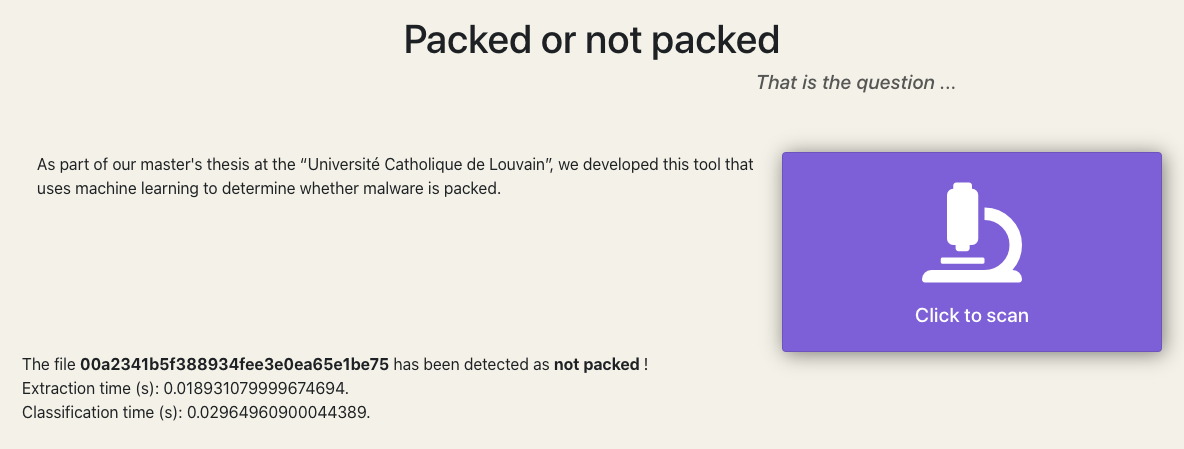
\includegraphics[width=\textwidth]{Figures/tools.png}
    \caption{Screenshot of the main page of the online detector}
    \label{fig:online_tool}
\end{figure}